\begin{frame}
	\myheading{Module 8.1 : Bias and Variance}
\end{frame}

\begin{frame}{}
			
	\begin{block}{}
				 	
		We will begin with a quick overview of bias, variance and the trade-off between them.
	\end{block}
\end{frame}
%%%%%%%%%%%%%%%%%%%%%%%%%%%%%%%%%%%%%%%%%%%%%%%%%%%%%%5
\begin{frame}
			
	\begin{columns}
				
		\begin{column}{0.4\textwidth}
							
			\begin{tikzpicture}
							
	\onslide<4->{\draw(-1,2) -- (4,1);}
	\onslide<6->{\draw[thick, blue] plot [smooth] coordinates {(2.55,2) (2.4,1.8) (2.3,1.5) (2.1,0.9) (2,0.6) (1.8,0.4) (1.7,0.3) (1.3,0) (1,0.3) (0.9,0.8) (0.9,1) (0.8,1.9) (0.6,2.2) (0.4,3.2) (0,3.5) (-0.3,3.2) (-0.5,2.5) };}
	\onslide<1->{ \draw plot[mark=+,only marks, mark options={color=red,scale=1}] coordinates { (-0.5,2.5) (-0.3,3.2) (0.4,3.2) (0.8,1.9) (0.9,1) (1,0.3) (2,0.6) (0.8,1.9) (2.4,1.8) };}
	\onslide<4->{\node[text width=4cm] at (5,1.3) {Simple};}
	\onslide<6->{\node[text width=4cm] at (4,0) {Complex};}
				
\end{tikzpicture}
			
			\justifying \onslide<1->{The points were drawn from a sinusoidal function (the true $f(x)$)}
		\end{column}
		\begin{column}{0.6\textwidth}
			
			
			\begin{itemize}
				\justifying
				\setlength\itemsep{1em}
				\item<1-> Let us consider the problem of fitting a curve through a given set of points
				\item<2-> We consider two models :
						
				\begin{align*}
					\onslide<3->{\substack{Simple\\(degree: 1)}~~~
					  & y=\hat{f}(x)=w_1x+w_0                   &   \\}
					\onslide<5->{\substack{Complex\\(degree: 25) }~~~
					  & y=\hat{f}(x)=\sum_{i=1}^{25} w_ix^i+w_0 & } 
				\end{align*} 
				\item<7->Note that in both cases we are making an assumption about how $y$ is related to $x$. We have no idea about the true relation $f(x)$
				\item<8->The training data consists of 100 points
			\end{itemize}
			
															
			
		\end{column}
	\end{columns}
\end{frame}
	
%%%%%%%%%%%%%%%%%%%%%%%%%%%%%%%%%%%%%%%%%%%%%%%%%%%55
\begin{frame}
	\begin{columns}
		\begin{column}{0.4\textwidth}
			\begin{tikzpicture}
							
	{\draw(-1,2) -- (4,1);}
	{\draw[thick, blue] plot [smooth] coordinates {(2.55,2) (2.4,1.8) (2.3,1.5) (2.1,0.9) (2,0.6) (1.8,0.4) (1.7,0.3) (1.3,0) (1,0.3) (0.9,0.8) (0.9,1) (0.8,1.9) (0.6,2.2) (0.4,3.2) (0,3.5) (-0.3,3.2) (-0.5,2.5) };}
	{ \draw plot[mark=+,only marks, mark options={color=red,scale=1}] coordinates { (-0.5,2.5) (-0.3,3.2) (0.4,3.2) (0.8,1.9) (0.9,1) (1,0.3) (2,0.6) (0.8,1.9) (2.4,1.8) };}
	{\node[text width=4cm] at (5,1.3) {Simple};}
	{\node[text width=4cm] at (4,0) {Complex};}
				
\end{tikzpicture}
			\justifying \onslide<1->{The points were drawn from a sinusoidal function (the true $f(x)$)}
								
		\end{column}
		\begin{column}{0.6\textwidth}
						
			\begin{itemize}
				\justifying
				\setlength\itemsep{1em}
				\item<1-> We sample 25 points from the training data and train a simple and a complex model
				\item<2-> We repeat the process `$k$' times to train multiple models (each model sees a different sample of the training data)
				\item<3-> We make a few observations from these plots
			\end{itemize}
		\end{column}
	\end{columns}
\end{frame}
%%%%%%%%%%%%%%%%%%%%%%%%%%%%%%%%%%%%%%%%%%%%%%%%%55
\begin{frame}
	\begin{columns}
		\begin{column}{0.4\textwidth}
											
			\begin{overlayarea}{\textwidth}{\textheight}
				\begin{figure}
					\includegraphics<1>[width=0.9\linewidth]{images/linear/0am.png}
					\includegraphics<2>[width=0.9\linewidth]{images/linear/1am.png}
					\includegraphics<3>[width=0.9\linewidth]{images/linear/2am.png}
					\includegraphics<4>[width=0.9\linewidth]{images/linear/3am.png}
					\includegraphics<5>[width=0.9\linewidth]{images/linear/4am.png}
					\includegraphics<6>[width=0.9\linewidth]{images/linear/5am.png}
					\includegraphics<7>[width=0.9\linewidth]{images/linear/6am.png}
					\includegraphics<8>[width=0.9\linewidth]{images/linear/7am.png}
					\includegraphics<9>[width=0.9\linewidth]{images/linear/8am.png}
					\includegraphics<10>[width=0.9\linewidth]{images/linear/9am.png}
					\includegraphics<11>[width=0.9\linewidth]{images/linear/10am.png}
					\includegraphics<12>[width=0.9\linewidth]{images/linear/11am.png}
					\includegraphics<13>[width=0.9\linewidth]{images/linear/12am.png}
					\includegraphics<14>[width=0.9\linewidth]{images/linear/13am.png}
					\includegraphics<15>[width=0.9\linewidth]{images/linear/14am.png}
					\includegraphics<16>[width=0.9\linewidth]{images/linear/15am.png}
					\includegraphics<17>[width=0.9\linewidth]{images/linear/16am.png}
					\includegraphics<18>[width=0.9\linewidth]{images/linear/17am.png}
					\includegraphics<19>[width=0.9\linewidth]{images/linear/18am.png}
					\includegraphics<20->[width=0.9\linewidth]{images/linear/19am.png}\\
					\includegraphics<24>[width=0.9\linewidth]{images/complex/0bm.png}
					\includegraphics<25>[width=0.9\linewidth]{images/complex/1bm.png}
					\includegraphics<26>[width=0.9\linewidth]{images/complex/2bm.png}
					\includegraphics<27>[width=0.9\linewidth]{images/complex/3bm.png}
					\includegraphics<28>[width=0.9\linewidth]{images/complex/4bm.png}
					\includegraphics<29>[width=0.9\linewidth]{images/complex/5bm.png}
					\includegraphics<30>[width=0.9\linewidth]{images/complex/6bm.png}
					\includegraphics<31>[width=0.9\linewidth]{images/complex/7bm.png}
					\includegraphics<32>[width=0.9\linewidth]{images/complex/8bm.png}
					\includegraphics<33>[width=0.9\linewidth]{images/complex/9bm.png}
					\includegraphics<34>[width=0.9\linewidth]{images/complex/10bm.png}
					\includegraphics<35>[width=0.9\linewidth]{images/complex/11bm.png}
					\includegraphics<36>[width=0.9\linewidth]{images/complex/12bm.png}
					\includegraphics<37>[width=0.9\linewidth]{images/complex/13bm.png}
					\includegraphics<38>[width=0.9\linewidth]{images/complex/14bm.png}
					\includegraphics<39>[width=0.9\linewidth]{images/complex/15bm.png}
					\includegraphics<40>[width=0.9\linewidth]{images/complex/16bm.png}
					\includegraphics<41>[width=0.9\linewidth]{images/complex/17bm.png}
					\includegraphics<42>[width=0.9\linewidth]{images/complex/18bm.png}
					\includegraphics<43->[width=0.9\linewidth]{images/complex/19bm.png}
								
								
				\end{figure}
			\end{overlayarea}						
										
		\end{column}
		\onslide<21->\begin{column}{0.6\textwidth}
		\begin{itemize}
			\justifying
			\setlength\itemsep{1em}
			\item<21-> Simple models trained on different samples of the data do not differ much from each other
			\item<22-> However they are very far from the true sinusoidal curve (under fitting)
												
			\item<44-> On the other hand, complex models trained on different samples of the data are very different from each other (high variance)
		\end{itemize}
		\end{column}
	\end{columns}
\end{frame}
%%%%%%%%%%%%%%%%%%%%%%%%%%%%%%%%%%%%%%%%%%%%%%%%%%%%55
	
\begin{frame}
	\begin{columns}
		\begin{column}{0.4\textwidth}
			\begin{figure}
				\justifying
				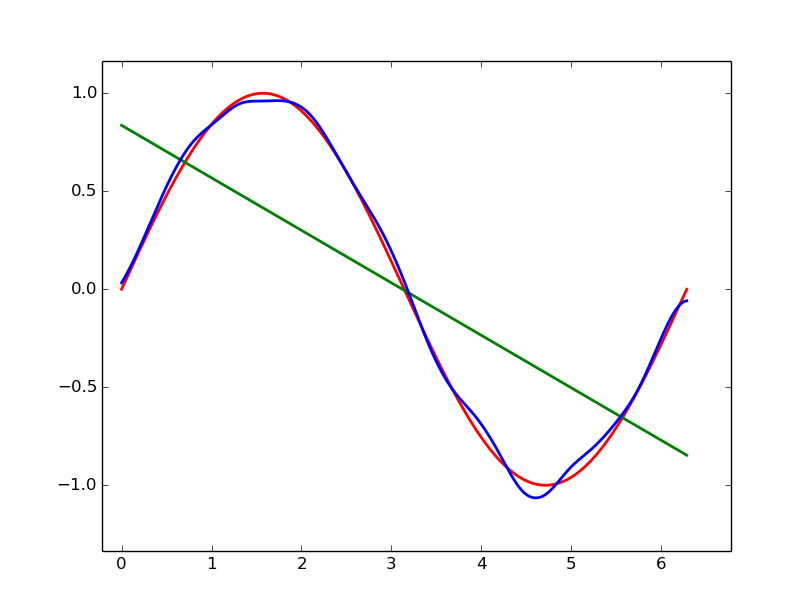
\includegraphics[width=0.9\linewidth]{images/combine}
				\caption{\underline{Green Line}: Average value of $\hat{f}(x)$ for the simple model\\
					\underline{Blue Curve}: Average value of $\hat{f}(x)$ for the complex model\\  
					\underline{Red Curve}: True model ($f$(x))}
				\label{fig:combine}
			\end{figure}
								
							
			%%%%%%%%% Blue line red curve black curve	
		\end{column}
					
		\begin{column}{0.6\textwidth}
			\begin{itemize}
				\justifying 						
				\setlength\itemsep{1em}
				\item<1-> Let $f(x)$ be the true model (sinusoidal in this case) and $\hat{f}(x)$ be our estimate of the model (simple or complex, in this case) then,
				\begin{align*}
					\text{Bias } & (\hat{f}(x))=E[\hat{f}(x)]-f(x) &   
				\end{align*}
				\item<2->$E[\hat{f}(x)]$ is the average (or expected) value of the model
									
				\item<3-> We can see that for the simple model the average value (blue line) is very far from the true value $f(x)$ (sinusoidal function)
				\item<4-> Mathematically, this means that the simple model has a high bias
				\item<5-> On the other hand, the complex model has a low bias
			\end{itemize}
		\end{column}
	\end{columns}
\end{frame}
%%%%%%%%%%%%%%%%%%%%%%%%%%%%%%%%%%%%%%%%%%%%%%%%%%%%%%%%%%
\begin{frame}
	\begin{columns}
		\begin{column}{0.4\textwidth}
			\begin{figure}
				\centering
				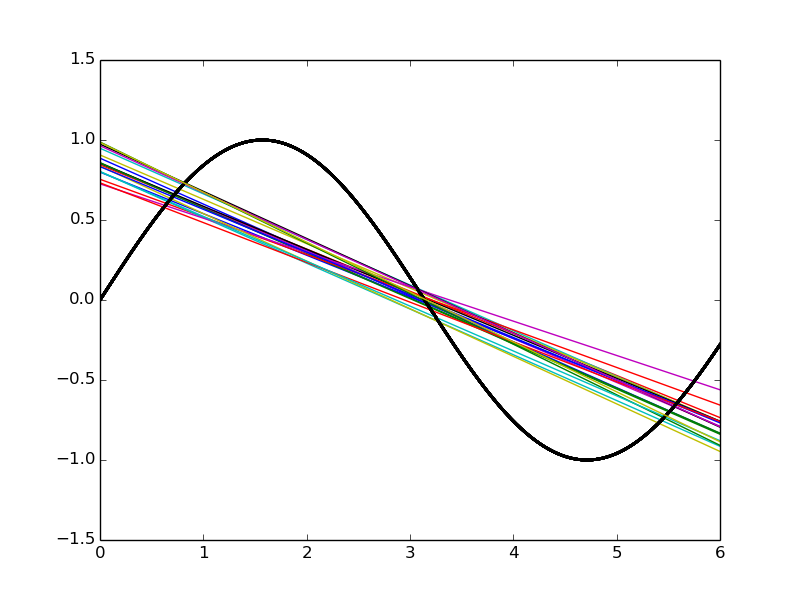
\includegraphics[width=0.9\linewidth]{images/linear/19am.png}\\
				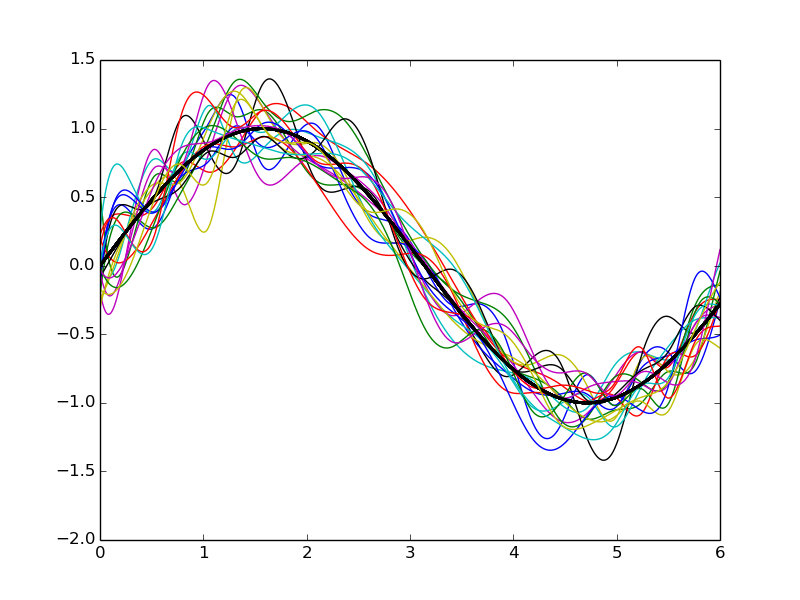
\includegraphics[width=0.9\linewidth]{images/complex/19bm.png}
				\caption{}
				\label{fig:simp}	
			\end{figure}
		\end{column}
		\begin{column}{0.6\textwidth}
			\begin{itemize}
				\justifying
				\setlength\itemsep{1em}
				\item<1-> We now define,\\
				\begin{align*}						\text{Variance } (\hat{f}(x))=E[(\hat{f}(x)-E[\hat{f}(x)])^2]\\\text{(Standard definition from statistics)}
				\end{align*}
										
				
										
				\item<2->Roughly speaking it tells us how much the different $\hat{f}(x)$'s (trained on different samples of the data) differ from each other
										
				\item<3-> It is clear that the simple model has a low variance whereas the complex model has a high variance
			\end{itemize}
		\end{column}
	\end{columns}
\end{frame}
%%%%%%%%%%%%%%%%%%%%%%%%%%%%%%%%%%%%%%%%%%%%%%%%%%%%%%%%%%%%%%%%%%%%%
\begin{frame}
	\begin{columns}
		\begin{column}{0.4\textwidth}
			\begin{figure}
				\centering
				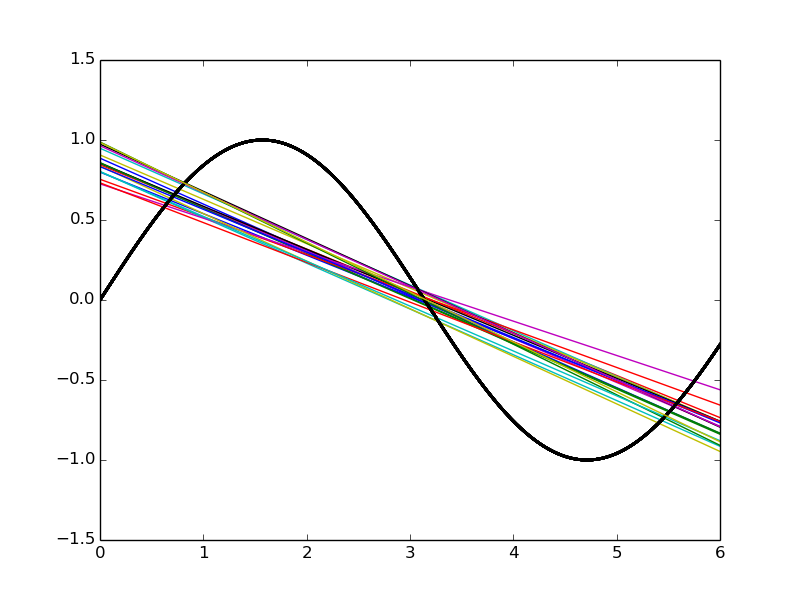
\includegraphics[width=0.9\linewidth]{images/linear/19am.png}\\
				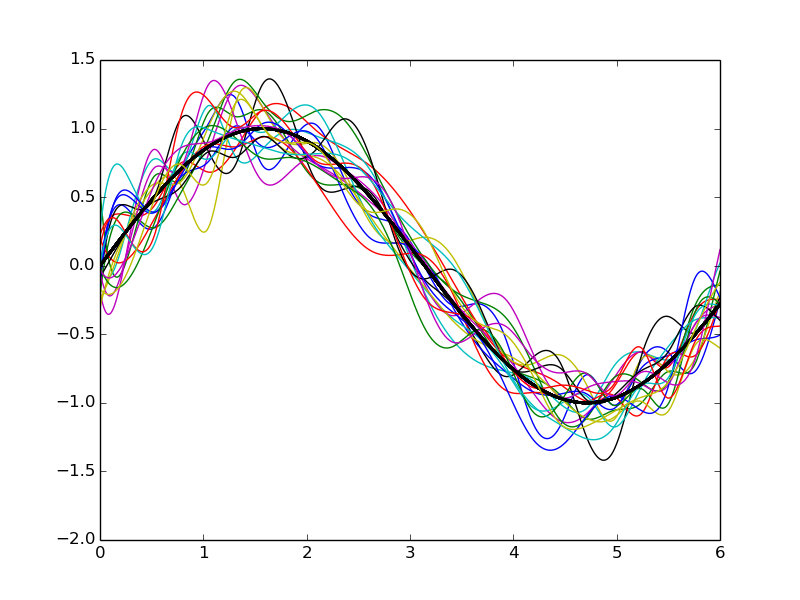
\includegraphics[width=0.9\linewidth]{images/complex/19bm.png}
				\caption{}
				\label{fig:simpl}
			\end{figure}
		\end{column}
		\begin{column}{0.6\textwidth}
			\begin{itemize}
				\justifying
				\item<1-> In summary (informally)
				\item<2-> Simple model: high bias, low variance					
				\item<3-> Complex model: low bias, high variance
				\item<4-> There is always a trade-off between the bias and variance
				\item<5-> Both bias and variance contribute to the mean square error. Let us see how,
			\end{itemize}
		\end{column}
	\end{columns}
\end{frame}
%%%%%%%%%%%%%%%%%%%%%%%%%%%%%%%%%%%%%%%%%%%%%%%%%%%%%%%%%%%%%%%%%%
